\documentclass{csmathnotes}

\udc{214.16}
\title{Задача извлечения сущностей в русскоязычном тексте}

\author{Аверина Мария Дмитриевна}
\position{магистр}
\affiliation{Ярославский государственный университет им. П.\,Г. Демидова}
\email{maverina518@gmail.com}

%\author{Дунаева Ольга Александровна}
%\position{к.ф.-м.н.}
%\affiliation{Ярославский государственный университет им. П.\,Г. Демидова}
%\email{olaydy@gmail.com}


\usepackage{diagbox}
\addbibresource{Averina.bib}


\begin{document}

\maketitle

\begin{abstract}
В статье приводятся общие подходы к извлечению сущностей из теста на русском языке. В статье рассмотрены способы извлечения признаков из текста, где в качестве метода классификации выбран \emph{CRF (conditional random fields)}. Построены различные признаки для классификация и выбраны наиболее оптимальные варианты для решения данной задачи. Данные на русском языке. Обучен классификатор \emph{CRF} для различных наборов признаков и алгоритмов оптимизации, выявлены наиболее эффективные признаки.
\end{abstract}

\keywords{NER, CRF, F1, токенизация, word2vec, fastText, нормализация слов}.

\section*{Введение}
Одна из важнейших задач – сбор и анализ статистических данных нормативных
документов – является достаточно трудоемкой для специалистов. На данный момент, в условиях повсеместного внедрения электронного документооборота, данная задача особенно актуальна. Автоматизация процесса анализа текстов – задачи распознавания именованных сущностей (\emph{named entity recognition}, \emph{NER})~\cite{base} – позволит оптимизировать работу многих специалистов как по временным, так и по качественным показателям.

\begin{figure}[h]
	\center{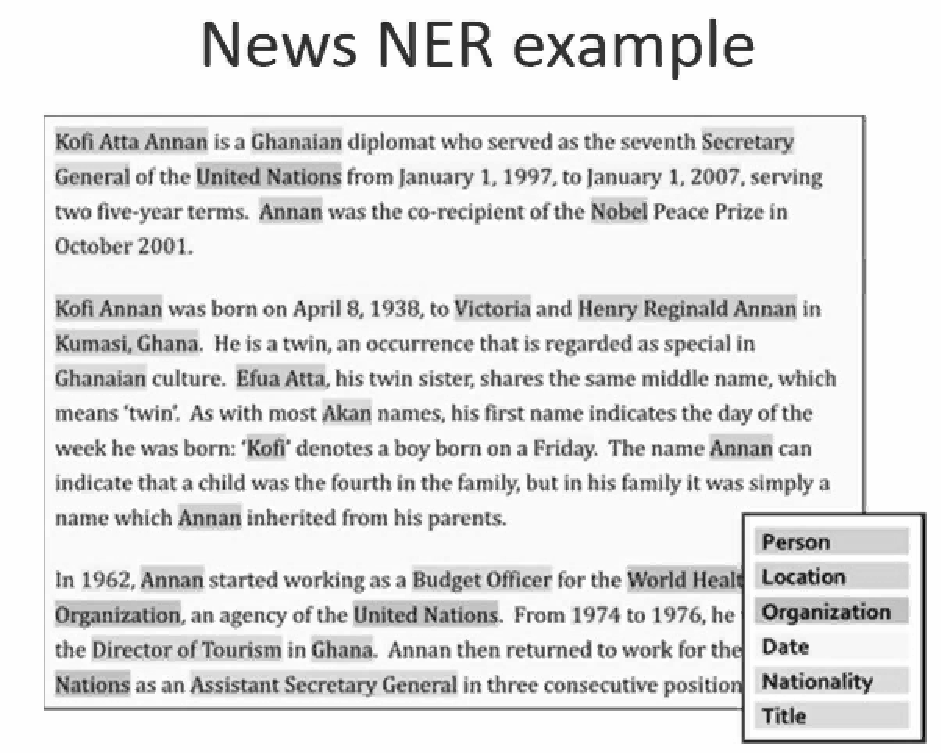
\includegraphics[scale=0.5]{1.pdf}}
	\caption{Результаты работы NER.}
	\label{fig:ner}
\end{figure}


Задача \emph{NER} (\emph{named entity recognition}) заключается в выделении определенных непрерывных фрагментов текста (сущности в тексте). Например, есть новостной текст, в котором необходимо выделить некоторый заранее зафиксированный набор сущностей (персоны, локации, организации, даты и т.д.). Таким образом необходимо определить, что участок текста «1 января 1997 года» является датой, «Кофи Аннан» – персоной, а «ООН» – организацией (~\ref{fig:ner}). 

\section*{Данные}
При разработке системы распознавания сущностей в русскоязычных текстах в качестве тестовых данных была использована выборка из 500 файлов открытой русскоязычной базы данных судебной статистики~\cite{CourtsData}. Такой выбор был сделан в силу большого количества доступных документов, а также соответствующего задаче характера текстов самих документов (наличие большого количества имён, дат, наименований, сумм и т.д.)

\subsection*{Предварительная обработка данных}
Первым этапом является предобработка данных: разбиение на слова, удаление ненужных символов, извлечение признаков слов. 
Токенизация — процесс разбиения текстового документа на отдельные слова, которые называются токенами.


Для начала, весь текст необходимо токенизировать~\cite{Ner}, при этом удаляются не несущие смысл символы и пробелы между цифрами. После весь текст приводится к нижнему регистру, а наличие заглавной буквы заносится в «словарь символов»(см. ниже).
При обработке данных необходимо выделить символы в начале и конце токена.  Например почта \emph{“v1@mail.com,”} будет разбита на \emph{“v1@”} и \emph{“mail.com,”}, где @ идентифицируется как слово-спецсимвол, а запятая добавляется в «словарь символов». Символ “@” , позволяет классифицировать строку как почтовый адрес. Используемые нами спецсимволы: @, \#, № ,\%, $/$.


Приведем список признаков в «словаре символов»:
\begin{itemize}
	\item первая буква большая, остальные маленькие,
	\item все буквы маленькие,
	\item все буквы большие,
	\item первая буква маленькая,
	\item наличие запятой или точки в конце или начале слова и т.д.
\end{itemize}

\subsection*{Формирование признаков}
\subsection*{Само слово, как признак}
Существует еще один признак - само слово(\emph{v}). Данный признак эффективен в паре со «словарем символов» при разнообразных данных(когда фамилия судьи не одна и та же) при обучении. Но он плохо подходит, если в обучающей выборке часто встречается одна и та же фамилия или одно и тоже название организации, поскольку классификатор «затачивается» на определенном слове.
\subsubsection*{Выделение признаков при помощи морфологического анализатора pymorphy}
Нормализация - приведение слов к «исходному» виду( лосями $\rightarrow$  лось, мыла $\rightarrow$ мыть, зеленого $\rightarrow$ зеленый). После нормализации число и род  можно отнести к отдельным признакам(n). Также возможно использовать часть речи(\emph{m})( существительное, предлог и т.д.), как признак для распознавания сущностей. В случае спецсимволов, после токенизации необходимо задавать каждому такому символу уникальные значения частей речи. Например, для символа \% морфологией будет \emph{PERCENT}.

 
\subsubsection*{Векторизация текстовых данных}
Процесс конвертации текста в векторы называется векторизацией~\cite{w2v} . Теперь после предобработки текста, необходимо представить его в числовом виде, то есть закодировать текстовые данные числами, которые в дальнейшем могут использоваться в обучении. Технология \emph{Word2Vec}(\emph{w}) работает с большими текстовыми данными и по определенным правилам присваивает каждому слову уникальный набор чисел — семантический вектор. В последнее время все более популярным становится подход к векторизации текста, при котором Word2Vec дополняется различными улучшениями. Два наиболее часто используемых улучшения — это \emph{GloVe} и \emph{fastText}(\emph{f}). \emph{FastText} исправляет недостаток \emph{Word2Vec}: если обучение модели начинается с прямого кодирования одного D-мерного вектора, то игнорируется внутренняя структура слов. Вместо прямого кодирования слов, \emph{fastText} предлагает изучать \emph{N-граммы} символов и представлять слова как сумму векторов \emph{N-грамм}.


\section*{Предсказание тегов при помощи CRF}
Наиболее  популярный способ для классификации именованных сущностей— \emph{CRF} (\emph{conditional random fields})~\cite{HabrCRF}. \emph{CRF} оптимизирует всю цепочку меток целиком, а не каждый элемент в этой цепочке.  Линейный \emph{CRF} хорошо подходит для решения задач сегментации и разметки последовательности, например:
\begin{itemize}
	\item автоматическое выделение ключевых слов из текстов,
	\item автоматическое выделение именованных сущностей(классификация сущностей),
	\item анализ тональности,
	\item автоматическое распознавание речи.
\end{itemize}


Сложность процесса обучения \emph{CRF} большая, а именно $O(mNTQ2nS)$ где:
\begin{itemize}
	\item \emph{m} — количество тренировочных итераций,
	\item \emph{N} — количество обучающих последовательностей (из обучающей коллекции),
	\item \emph{T} — средняя длина обучающей последовательности,
	\item \emph{Q} — количество выходных классов,
	\item \emph{n} – количество признаков в обучающей матрице,
	\item \emph{S} – время работы алгоритма оптимизации на каждом шаге. 
\end{itemize}


\emph{CRF} может учитывать любые особенности и взаимозависимости в исходных данных.
\begin{itemize}
	\item Один из лучших методов для \emph{NER},
	\item Очень долго обучается,
	\item Хорошо работает в связке с рекуррентными нейросетями, моделирует совместное распределение на всей последовательности выходов сети одновременно.
\end{itemize}

На практике вычислительная сложность обучения(время обучения) \emph{CRF} даже выше за счет всевозможных дополнительных операций таких, как сглаживание, преобразование данных из формата в формат и т.д. Отметим, что при увеличении количества признаков(учитывание признаков соседних слов) время обучения значительно увеличиться. 

\section*{Метрика F1}
После того как классификатор обучен необходимо оценить качество его работы. Например, метрики \emph{Precision(P}) и \emph{Recall(R)} дают исчерпывающую характеристику классификатора. Но, как правило при построении классификаторов приходится все время балансировать между двумя этими метриками. Если повысить \emph{Recall}, делая классификатор более «оптимистичным», это приводит к падению Precision из-за увеличения числа ложно-положительных ответов. Если же наоборот классификатор делать более «пессимистичным», то при росте \emph{Precision} это вызовет одновременное падение \emph{Recall} из-за отбраковки какого-то числа правильных ответов. Поэтому удобно для характеристики классификатора использовать одну величину, так называемую метрику \emph{F1}(среднегармонической между \emph{Recall} и \emph{Precision}):

\begin{equation}\label{eq:f1}
F1 = 2\frac{P R}{P + R} 
\end{equation}

Для оценки результатов будем использовать меру \emph{F1}, но \emph{precision} и \emph{recall} будем считать, объединяя соседние слова с одним тегом в одну тегированную сущность, Поскольку одна сущность может состоять из нескольких токенов, то стоит при оценивание качества учитывать ее целиком. 

\section*{Результаты}
Рассмотрим результаты тестирования на данных судебных протоколов: наилучшего качества классификации можно добиться за счет подбора параметров классификатора. Необходимо выбрать наиболее эффективный и быстрый оптимизатор для \emph{CRF}. В таблице ~\ref{tabl:table1} приведен анализ оптимизаторов, при фиксированном наборе признаков.
\begin{table}[h]
	\begin{center}
		\begin{tabular}{|p{3cm}|p{1.3cm}|p{1.5cm}|p{1.5cm}|p{2.5cm}|}
			\hline
			Алгоритм оптимизации &  Долгое время работы & Лучший результат & \emph{F1} на худшей сущности & Примечания \\
			\hline
			\emph{lbfgs} - градиентный спуск с использованием метода 
			L-BFGS & + & $1$ & $0.7$ & время обучения более $5$ часов  \\
			\hline
			\emph{l2sgd} - стохастического  градиентного спуска  с регуляризации L2 & + & $1$  & $0$ & классифицирует все, как самый объемный класс \\
			\hline
			\emph{pa} - усредненный персептрон & - & $1$  & $0.45$ & время работы не более $30$ минут \\
			\hline
			\emph{ap} - Passive Aggressive & - & $0.83$ & $0.24$  & - \\
			\hline
			\emph{arow} - адаптивная регуляризация  & - & $0.79$ & $0.31$  & - \\
			\hline
		\end{tabular}
	\end{center}
	\caption{\label{tabl:table1}Сравнительный анализ алгоритмов оптимизации.}
\end{table}

Как видно из таблицы ~\ref{tabl:table1} лучший результат показали алгоритмы pa и \emph{lbfgs}, но поскольку алгоритм \emph{lbfgs}  достаточно трудоемкий, в качестве оптимального был выбран алгоритм \emph{pa}.


\begin{table}[!h]
	\begin{center}
		\begin{tabular}{|p{3.1cm}|p{2.5cm}|p{2.5cm}|p{2.5cm}|}
			\hline
			\diagbox[width=9.9em]{Признаки}{Оптимизатор} &  pa & l2sgd & lbfgs \\
			\hline
			$(r3, v3)$ & - & - & 
			best:\newline  doc num  $0.993$ \newline
			worst:\newline defendant  $0.751$ \newline
			time fit:\newline  $5.55.36$ \\
			\hline
			$(r3, v1)$ & best: \newline judge $0.906$ \newline
			worst: \newline defendant   $0.455$ 
			\newline time fit:  \newline $0.07.58$
			& best:\newline judge  $0.867$ \newline
			  worst: \newline defendant    $0.116$ \newline
			  time fit:\newline $0.4.11$
			& best:\newline   doc num  $0.973$ \newline
			  worst:\newline defendant  $0.685$\newline
			  time fit:\newline  $3.32.49$ \\
			\hline
			$(w1, v1, m1)$ 
			& best:\newline    court   $0.827$ \newline
			worst: \newline defendant   $0.331$ \newline
			time fit:\newline $0:05:20.747838$ \newline
			& best: \newline judge    $0.751$ \newline
			  worst: \newline court  $0.013$ \newline
			  time fit:\newline $0:3:14$
			& best:\newline  judge $0.971$\newline
			  worst: \newline defendant  $0.541$\newline
			  time fit:\newline $3.03.01$\\
			\hline
			$(r3, m3)$
			& best: \newline judge $0.692$ \newline
			worst: \newline payment fine $0.412$ \newline
			time fit: \newline  $0.33.58$
			& best:\newline   date court   $0.746$ \newline
			 worst: \newline court $0.126$ \newline
			 time fit: \newline $0.12.11$
			& best: \newline   judge $0.818$ \newline
			  worst:\newline defendant $0.285$ \newline 
			  time fit: \newline $3.58.24$\\
			\hline
		\end{tabular}
	\end{center}
	\caption{\label{tabl:table2}Сравнительный анализ F-меры.}
\end{table}

Заметим, что наименьший разброс \emph{f1}  принимает при признаках $(r3,v3)$ с оптимизатором \emph{lbfgs}, при этом демонстрируя достаточно высокий средний результат(таблица ~\ref{tabl:table2}). Однако, время обучения такой модели более пяти часов. При необходимости уменьшить время обучения наиболее оптимальным решением будет обучение модели на признаках $(r3,v1)$ с оптимизатором \emph{pa}.

\section*{Заключение}
Подведем итоги. Нами была решена задача морфологической классификации, которая достаточно трудна для русского языка так, как ни в одном языке нет столько склонений, спряжений и т. д. 


В данной работе проведен сравнительный анализ алгоритмов оптимизации, различных наборов признаков. Алгоритм \emph{pa} с признаками $(r3, v1)$ показал наилучший результат по времени и \emph{F1}  в совокупности. Алгоритм \emph{lbfgs}  с признаками $(r3, v3)$ продемонстрировал лучший результат по \emph{F1}, но оказался трудоемким и долгообучаемым. Стоит отметить, что лучший результат показал алгоритм \emph{pa} по времени. Но для более точного предсказания будет необходимо использовать \emph{lbsg}.


Для дальнейшего улучшения результатов планируется выделять еще новые признаки, а также можно попробовать использовать другие методы классификации и усовершенствование архитектуры классификатора на основе \emph{biLSTM} и \emph{BERT}

\printbibliography

\end{document}
